\documentclass["../Cours.tex"]{subfiles}

\begin{document}
\chapitre{Réciproques}

\partie{Réciproque du théorème de Pythagore}

\theoreme{Si, dans un triangle, le carré de la longueur du plus grand côté est égal à la somme des carrés des longueurs des deux autres côtés, alors le triangle est rectangle.}{}

\exemple{
\begin{center}
    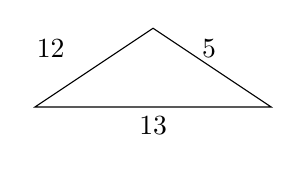
\begin{tikzpicture}
        \draw (0,0) -- (3,0) -- (1.5,1) -- cycle;
        \node[below] at (1.5,0) {13};
        \node[above right] at (2,0.5) {5};
        \node[above left] at (0.5,0.5) {12};
    \end{tikzpicture}
\end{center}
\begin{itemize}
    \item D'une part, $13^2 = 169$\\
    D'autre part, $12^2+5^2 = 144+25=169$
    \item D'après la réciproque du théorème de Pythagore
    \item Le triangle est rectangle
\end{itemize}
}

\partie{Réciproque du théorème de Thalès}

\illustration{
\begin{center}
    \begin{tikzpicture}
        
    \end{tikzpicture}
\end{center}
}




\end{document}